\subsection{Flowing to the 'IR' (long distances)} 
Imagine we only care about predictions at on scales
$ L \gg a $. Then, we can write a theory 
with a new cutoff given by 
\[
 \Lambda' = \frac{ \Lambda }{ \epsilon }, \quad \epsilon > 1 
\] This means that all fourier modes $ \frac{1}{ L } \leq | \vec{k} | \leq \Lambda $
We can expand Fourier modes as 
\[
\phi_{ \vec{k} }  = \phi_{\vec{k}}^-  + \phi_{ \vec{k} } ^ + 
\] The $ \phi_{ \vec{k} }^-$ are low frequency modes with 
\[
 \phi_{ \vec{k} }^ -  = \begin{cases}
	 \phi_{ \vec{k} } &  | \vec{k} | \leq \Lambda ' \\
	 0 & \text{ otherwise }
 \end{cases}
\] And our $ \phi_{ \vec{k} } ^ + $ are our high frequency 
terms with 
\[
 \phi_{ \vec{k} }^  +  = \begin{cases}
	 \phi_{ \vec{k}  } & \Lambda ' < \| \vec{k} \| < \Lambda \\
	 0 & \| k \| \geq \Lambda 
 \end{cases}
\]  
We can write out our free energy 
in terms of this fourier mode split, so that 
\[
	F [ \phi _{ \vec{k}  } ] = F_ 0 [ \phi_{ \vec{k} }^ - ]  + F_ 0 [ \phi_{ \vec{k} } ^ +   ] + F_ I [ \phi_{ \vec{k} } ^ + , \phi_{ \vec{k} } ^ - ]  
\]  The final term in this expression can be 
interpreted as an interaction between long and short length scales 
in the Fourier modes. 
We can then write out our partition function as
\[
	\mathcal{ Z} =  \int \prod_{ k <  \Lambda  } d \phi_{ \vec{k}} e^{  - F }  
\] However, the upshot of this is that 
now we can decompose $ F $ into the high and low frequency modes 
which we were derived earlier.
We have that
\[
	\mathcal{ Z } = \int \prod_{ k <  \Lambda ' } d \phi_{ \vec{k} }^- e^{  - F_0 [ \phi _{ \vec{k}} ^-]} \int \prod_{ \Lambda ' <  k < \Lambda} d \phi_{ \vec{k} } ^ + e^{  - F_ 0 [ \phi_{ \vec{k} } ^ +  ] } e^{  - F_ I [ \phi_{ \vec{k} } ^ + , \phi_{ \vec{k} } ^ - ]}
\] But the upshot of writing things out 
like this is that we can then write out an 'effective' 
action which only concerns integrals 
from our product of low frequency Fourier modes. In 
other words, we have that 
\[
	\mathcal{ Z } = \int d \phi_{ \vec{k}  } ^ - e^{  -F' [ \phi_{ \vec{k} } ^ -  ] }, \quad e^{  - F' [ \phi_{ \vec{k} } ^ - ]} = e^{ - F_ 0 [ \phi_{ \vec{k} } ^ -  ] } \int \prod_{ \Lambda ' < k < \Lambda } d \phi_{ \vec{k} } ^ +   e^{  - F_ 0 [ \phi_{ \vec{k} } ^ +  ] } e^{  - F_ I [ \phi_{ \vec{k} } ^ + , \phi_{ \vec{k} } ^ - ]}
\] 
%\begin{align*}
  % 	\mathcal{ Z } &=  \int \prod_{ \| k \| \le \Lambda ' }  e^{  - F_0 [ \phi_{ \vec{k} ^ -  }  ]  } \int \prod_{ \Lambda < k < \Lambda ' } d \phi_{ \vec{k} } ^ + e^{  - F_0 [ \phi_{ \vec{k} } ^ - ]   } e^{  - F_{ I } [ \phi_{ \vec{k} } ^ - , \phi_{ \vec{k} } ^ + ]}\\
% 	     &=  \int_{ k < \Lambda' } d \phi_{ \vec{k} } ^ - e^{  - F ' [ \phi_{\vec{k} } ^ - ] } 

%\end{align*}
We define $ F' $ as the Wilsonian effective action.
In other words, 
$ F '$  is now a shifted version of our free theory, giving that 
\[
	F ' [ \phi ] = \int d^ d x \, \left[  \frac{1}{2 } \gamma ' ( \nabla \phi ) ^ 2 + \frac{1}{2 } \mu^{ ' 2 } \phi ^ 2 + g ' \phi ^ 4  \right] 
\] We cannot direction compare $ F ' [ \phi ] $ with $ F [ \phi ] $
because they have  \textbf{different cutoff } regimes in 
our new theory. 
Nonetheless, there's a trick we can do to put 
these theories on the same footing. 
To do this, we use a technique called 
momentum rescaling, by rescaling momenta such that 
\[
 \vec{k} ' = \zeta \vec{k}, \quad \vec{x} ' = \frac{\vec{x} }{ \zeta }, \quad \zeta = \frac{ \Lambda }{ \Lambda ' } 
\] When we do this, we have that $ \Lambda' $ is rescaled to $ \Lambda$. 
Finally, for convention's sake, we can do a field rescaling to 
absorb  $ \gamma ' $ into the definition of $ (  \nabla \phi ) ^ 2 $. 

Now, our new action $ F_{ \zeta } $ can be written in terms of this new 
rescaling parameter. We hence write 
\[
	F_{ \zeta } [ \phi_{ \vec{k} } ^ - ] = \int d^ d x \left[  \frac{1}{2 } ( \nabla \phi' ) ^ 2 + \frac{1}{2 } \mu ^ 2 ( \zeta ) \phi ^{ ' 2 } + g ( \zeta ) \phi ^{ ' 4 }  \right] 
\] We have a diagram with one axis being $ g_k $ and on another axis we 
have $ g_ i $, with flows across them which represents some coupling constants. 
We flow in the direction of increasing $ \zeta  $. 

\begin{figure}[h]
	\centering
	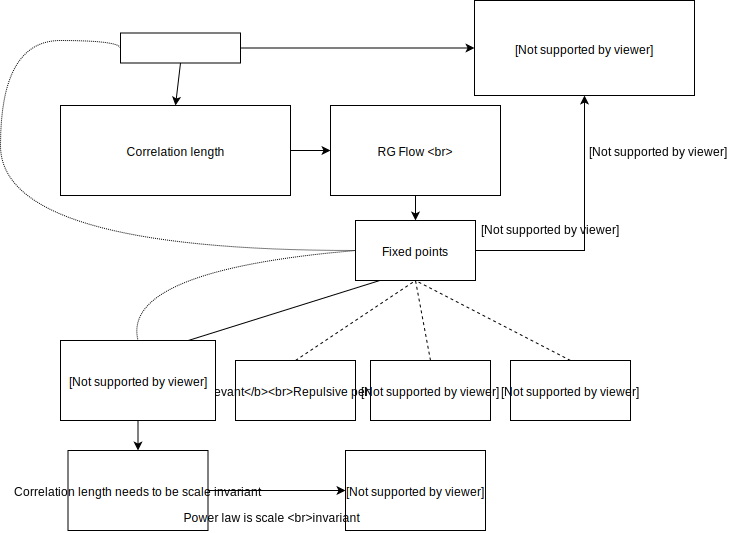
\includegraphics[scale=0.6]{figures/rg_flow_1.png}
	\caption{A schematic on how fixed points in RG flow mean different behaviours for temperatures}
\end{figure}

